\documentclass[10.5pt]{article}
\usepackage{amsmath, amsfonts, amssymb,amsthm}
\usepackage{graphicx}
\usepackage[includeheadfoot]{geometry} % For page dimensions
\usepackage{fancyhdr}
\usepackage{enumerate} % For custom lists

\fancyhf{}
\lhead{Math 425hw5}
\rhead{Tighe McAsey - 37499480}
\pagestyle{fancy}

% Page dimensions
\geometry{a4paper, margin=1in}

\theoremstyle{definition}
\newtheorem{pb}{}

% Commands:

\newcommand{\set}[1]{\{#1\}}
\newcommand{\abs}[1]{\lvert#1\rvert}
\newcommand{\norm}[1]{\lvert\lvert#1\rvert\rvert}
\newcommand{\gen}[1]{\langle #1 \rangle}
\newcommand{\tand}{\text{ and }}
\newcommand{\tor}{\text{ or }}
\newcommand{\vp}{\varphi}
\newcommand{\R}{\text{Re}}
\newcommand{\I}{\text{Im}}
\newcommand{\parx}{\frac{\partial}{\partial x}}
\newcommand{\pary}{\frac{\partial}{\partial y}}
\newcommand{\parz}{\frac{\partial}{\partial z}}

\begin{document}
    \begin{pb}
        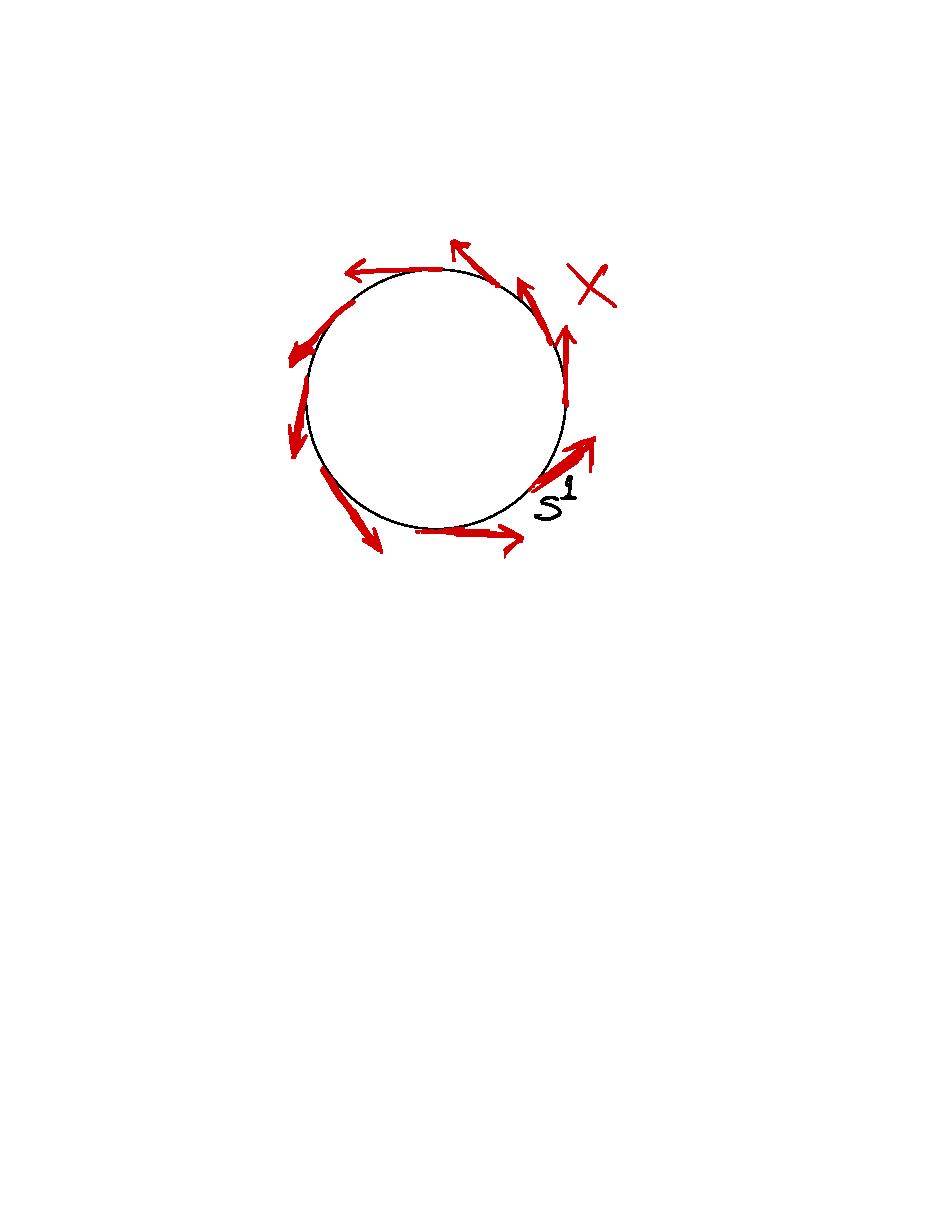
\includegraphics[scale=1]{graphics/Tighe.pdf}
        \newpage

        We can rewrite each \(x,y \in S^1\) as \((\cos(\theta),\sin(\theta))\) for \(\theta \in [0,2\pi)\) Define \(\gamma(t) = (\cos(\theta + t),\sin(\theta + t))\), then we have
        \(\gamma(0) = (\cos(\theta),\sin(\theta)) = (x,y)\) and \(\left.\frac{d}{dt}\right\vert \gamma(t) = (-\sin(\theta),\cos(\theta)) = (-y,x)\), so this path corresponds to the vector field \(X\).

        Now we compute \(X\vert_U\), we get

        \begin{align*}
            X\vert_U &= \frac{d}{dt}\vert_{t=0} \gamma(t)(u) \frac{\partial}{\partial u}= \frac{d}{dt}\vert_{t=0} \frac{\cos(\theta + t)}{1 - \sin(\theta + t)} \frac{\partial}{\partial u}
            = \left.\frac{-(1-\sin(\theta+t))\sin(\theta+t)+\cos^2(\theta+t)}{(1-\sin(\theta+t))^2}\right\vert_{t=0} \frac{\partial}{\partial u}\\
            &= \left.\frac{-\sin(\theta + t) + \cos^2(\theta+t) + \sin^2(\theta + t)}{1 - \sin(\theta + t)^2}\right\vert_{t=0} \frac{\partial}{\partial u}
            = \frac{1}{1 - \sin(\theta)} \frac{\partial}{\partial u}  = \frac{1}{1 - y} \frac{\partial}{\partial u}
        \end{align*}
        On \(U\) we have the inverse sterographic projection is \(u \mapsto (\frac{2u}{u^2 + 1}, \frac{u^2 - 1}{u^2 + 1})\). So we get that
        \begin{align*}
            X\vert_U = \frac{1}{1 - y} \frac{\partial}{\partial u} = \frac{1}{1 - \frac{u^2 - 1}{u^2 + 1}} \frac{\partial}{\partial u} = \frac{u^2 + 1}{2} \frac{\partial}{\partial u}
        \end{align*}
        Finally, we compute \(X\vert_{\tilde{U}}\). First note that \(\frac{\partial \tilde{u}}{\partial u} = \frac{\partial}{\partial u} \frac{1}{u} = \frac{-1}{u^2} = -\tilde{u}^2\)
        \begin{align*}
            X\vert_{\tilde{U}} = \frac{\partial \tilde{u}}{\partial u} X = -\tilde{u}^2 \frac{u^2 + 1}{2} \frac{\partial}{\partial \tilde{u}} 
            = -\frac{1 + \tilde{u}^2}{2} \frac{\partial}{\partial \tilde{u}}
        \end{align*}
        
        
        % \[\gamma(t) := u + t(\frac{2u}{u^2 + 1} - \frac{u^2 - 1}{u^2 + 1})\]
        % Then it is immediate that \(\gamma(0) = u\), and \(\frac{d}{dt}\vert_{t=0} \gamma(t) = \frac{2u}{u^2 + 1} - \frac{u^2 - 1}{u^2 + 1}\).
        % This corresponds exactly to \(X\) in cartesian coordinates, given the inverse coordinate function shown previously.

        % Then we have
        % \[X\vert_U = \frac{2u}{u^2 + 1} - \frac{u^2 - 1}{u^2 + 1} \frac{\partial}{\partial u}\]
        % Now we compute \(\tilde{X}\), we have \(\frac{\partial \tilde{u}}{\partial u} = \frac{\partial}{\partial u} \frac{1}{u} = \frac{-1}{u^2} = -\tilde{u}^2\).
        % Rewriting using \(\tilde{u} = \frac{1}{u}\), we get 
        % \(\frac{2u}{u^2 + 1} - \frac{u^2 - 1}{u^2 + 1} = \frac{2 \tilde{u}}{1 + \tilde{u}^2} - \frac{1-\tilde{u}^2}{1 + \tilde{u}^2}\)
        % \begin{align*}
        %     \tilde{X}\vert_{\tilde{U}} = -\tilde{u}^2 \left(\frac{2\tilde{u}}{\tilde{u}^2 + 1} - \frac{1 - \tilde{u}^2}{1 + \tilde{u}^2}\right)
        % \end{align*}
    \end{pb}
    \begin{pb}
        Define
        \begin{align*}
            \Theta_t: (e^{i\theta_1}, e^{i\theta_2}) \mapsto (e^{i(\theta_1 + at)},e^{i(\theta_2 + bt)})
        \end{align*}
        To show it is a flow, \(\Theta_0(\theta_1, \theta_2) = (\theta_1, \theta_2)\)
        \[\Theta_t \circ \Theta_s (e^{i\theta_1}, e^{i\theta_2}) = \Theta_t(e^{i(\theta_1 + as)},e^{i(\theta_2 + bs)}) 
        = (e^{i(\theta_1 + as + at)},e^{i(\theta_2 + bs + bt)}) = \Theta_{t+s} (e^{i\theta_1}, e^{i\theta_2})\]
        Equipping each copy of \(S^1\) with the standard charts, gives us 4 charts \(U_i\), smoothness is clear, since in any chart, 
        we have \(\Theta_t\vert_U : (\theta_1,\theta_2) \mapsto (\theta_1+ta,\theta_2+tb)\) is smooth. Then in any of the charts, we have
        \begin{align*}
            \frac{d}{dt}\vert_{t=0} \Theta_t(\theta_1,\theta_2) = \frac{d}{dt}\vert_{t=0} \theta_1 + at \frac{\partial}{\partial \theta_1} + \frac{d}{dt}\vert_{t=0} \theta_2 + bt \frac{\partial}{\partial \theta_2}
            = a\frac{\partial}{\partial \theta_1} + b\frac{\partial}{\partial \theta_2}
        \end{align*}
    \end{pb}
    \begin{pb}
        \textbf{(a)}
        We can compute
        \begin{align*}
            \hat{\theta_t}^{-1} = \begin{bmatrix} 1 & 0 & 0 \\ 0 & \cos t & -\sin t \\ 0 & \sin t & \cos t \end{bmatrix}
        \end{align*}
        To show smoothness, we show smoothness between two of the hemisphere charts, the other ones follow similarly. We take the charts \(U = \set{x > 0} \cap S^2\) and \(\tilde{U} = {y > 0}\cap S^2\), then
        \begin{align*}
            \tilde{\varphi}\hat{\theta_t}\varphi^{-1}(u,v) = \tilde{\varphi}\hat{\theta_t} \begin{bmatrix}\sqrt{1-u^2-v^2}\\u\\v\end{bmatrix} 
            = \tilde{\varphi}\begin{bmatrix} \sqrt{1-u^2-v^2}\\ u\cos t + v\sin t \\ -u\sin t + v\cos t \end{bmatrix} = \begin{bmatrix} \sqrt{1-u^2-v^2} \\ -u\sin t + v\cos t \end{bmatrix}
        \end{align*}
        Which is smooth since it is infinitely differentiable in \(u,v\) (note \(u^2 + v^2 \neq 1\) by choice of chart). We check smoothness of \(\hat{\theta_t}^{-1}\) on the same charts
        \begin{align*}
            \tilde{\varphi}\hat{\theta_t}^{-1}\varphi^{-1}(u,v) = \tilde{\varphi}\hat{\theta_t}^{-1} \begin{bmatrix}\sqrt{1-u^2-v^2}\\u\\v\end{bmatrix} 
            = \tilde{\varphi}\begin{bmatrix} \sqrt{1-u^2-v^2}\\ u\cos t + -v\sin t \\ u\sin t + v\cos t \end{bmatrix} = \begin{bmatrix} \sqrt{1-u^2-v^2} \\ u\sin t + v\cos t \end{bmatrix}
        \end{align*}

        \textbf{(b)} For any point \((x,y,z) \in S^2\), we can compute
        \begin{align*}
            X = \frac{d}{dt}\vert_{t=0} \hat{\theta_t}(x,y,z) = \frac{d}{dt}\vert_{t=0} \begin{bmatrix} x \\ y\cos t + z\sin t \\-y\sin t + z\cos t  \end{bmatrix}
            = \left.\begin{bmatrix}
                0 \\ -y \sin t + z\cos t \\ -y\cos t - z\sin t
            \end{bmatrix}\right\vert_{t=0} = \begin{bmatrix} 0 \\ z \\ -y \end{bmatrix}
        \end{align*}
        Then \(X = 0\) only at \(N = (1,0,0) \tand S = (-1,0,0)\).
    \end{pb}
    \begin{pb}
        % X = z\pary - y\parz
        % Y = x\parz - z\parx
        % Z = y\parx - x\pary
        \textbf{(a)}
        To show injectivity, assume that
        \(aX + bY + cZ = qX + rY + sZ\), Then we will show \(a = q, b = r, c = s\).
        \begin{align*}
            0 &\equiv (a-q)X + (b-r)Y + (c-s)Z = (a-q)(z\frac{\partial}{\partial y} - y\frac{\partial}{\partial z}) + (b-r)(x \frac{\partial}{\partial z} - z \frac{\partial}{\partial x}) +
            (c-s)(y \frac{\partial}{\partial x} - x \frac{\partial}{\partial y})\\
            &= (-z(b-r) + y(c-s))\frac{\partial}{\partial x} + (z(a-q)-x(c-s))\frac{\partial}{\partial y} + (-y(a-q) + x(b-r))\frac{\partial}{\partial z}
        \end{align*}
        So that setting \((x,y,z) = (1,0,0)\) we get \(c - s = 0 = b-r\) by linear independence, and setting \((x,y,z) = (0,1,0)\) we get \(a-q = 0\), hence proving injectivity.
        We have the correspondance \(X \leftrightarrow i\), \(Y \leftrightarrow j\) and \(Z \leftrightarrow k\). We only need verify that the bracket matches the multiplication rules of cross product,
        since bilinearity and antisymmetry come from bracket properties, we simply check that \([X,Y] = Z, [Y,Z] = X \tand [Z,X] = Y\). Computation below:
        \begin{align*}
            [X,Y] &= (z\pary - y\parz)x\parz + (z\pary - y\parz)(-z\parx) - \left((x\parz - z\parx)z\pary + (x\parz - z\parx)(-y\parz)\right) \\
            &= y \parx - x\pary = Z \\
            [Y,Z] &= (x\parz - z\parx)y\parx + (x\parz - z\parx)(-x\pary) - \left((y\parx - x\pary)x\parz + (y\parx - x\pary)(-z\parx)\right) \\
            &= z\pary - y\parz = X \\
            [Z,X] &= (y\parx - x\pary)z\pary + (y\parx - x\pary)(-y\parz) - \left((z\pary - y\parz)y\parx + (z\pary - y\parz)(-x\pary)\right) \\
            &= x\parz - z\parx = Y
        \end{align*}


        \textbf{(b)} take \(\theta_t: (x,y,z) \mapsto (x\cos t - z\sin t,y,z \cos t + x \sin t)\). Then we can verify immediately that
        \begin{align*}
            \frac{d}{dt}\vert_{t=0} \theta_t: (x,y,z) = (-x\sin t - z\cos t)\vert_{t=0}\frac{\partial}{\partial x} + (-z\sin t + x \cos t)\vert_{t=0} \frac{\partial}{\partial z} 
            = -z \frac{\partial}{\partial x} + x \frac{\partial}{\partial z} = Y
        \end{align*}
        This is clearly smooth, since it is a trig polynomial. To verify it is a flow, we need only verify \(\theta_t \circ \theta_s = \theta_{t + s}\) (I will omit the y-coordinate for brevity)
        \begin{align*}
            &\theta_a \circ \theta_b(x,y,z) = \theta_a (x \cos b - z \sin b, z \cos b + x \sin b) \\
            &= (\cos a(x\cos b - z\sin b) - \sin a (z\cos b + x\sin b), \cos a (z \cos b + x \sin b) + \sin a (x \cos b - z \sin b)) \\
            &= (x (\cos a \cos b - \sin a \sin b) - z(\cos a \sin b + \cos b \sin a), x(\cos a \sin b + \cos b \sin a) + z(\cos a \cos b - \sin a \sin b)) \\
            &= (x\cos(a+b) - z\sin(a+b),x\sin(a+b) + z\cos(a+b)) \\
            &= \theta_{a+b}(x,y,z)
        \end{align*}
        Here I used the sum of angle formulas \(\cos a \cos b - \sin a \sin b = \cos(a+b) = \cos(a+b) \tand \cos a \sin b + \cos b \sin a = \sin(a+b)\) for the second last equality.
        Hence this is the unique flow corresponding to \(Y\) (uniqueness of flow proven in lecture).
    \end{pb}
\end{document}